\documentclass[runningheads,a4paper]{llncs}

\usepackage{mathtools}
\usepackage{amssymb}
\setcounter{tocdepth}{3}
\usepackage{graphicx}
\usepackage{wrapfig}
\usepackage[caption=false]{subfig}
\usepackage{tikz}
\usepackage{pgfplots}
\pgfplotsset{compat=1.9}

\usepackage{url}
\usepackage{algpseudocode}
\usepackage{algorithm}
\usepackage{algorithmicx}

%\captionsetup[figure]{width=.85\textwidth}
%\captionsetup[subfigure]{width=.45\textwidth}
  
\newcommand{\keywords}[1]{\par\addvspace\baselineskip
\noindent\keywordname\enspace\ignorespaces#1}

%To economize paper
%\textwidth=190mm
%\textheight=250mm
%\topmargin=-20mm
%\oddsidemargin=-15mm
%\evensidemargin=-15mm


\begin{document}

\algnewcommand\algorithmicswitch{\textbf{switch}}
\algnewcommand\algorithmiccase{\textbf{case}}
\algnewcommand\algorithmicassert{\texttt{assert}}
\algnewcommand\Assert[1]{\State \algorithmicassert(#1)}
% New "environments"
\algdef{SE}[SWITCH]{Switch}{EndSwitch}[1]{\algorithmicswitch\ #1\ \algorithmicdo}{\algorithmicend\ \algorithmicswitch}
\algdef{SE}[CASE]{Case}{EndCase}[1]{\algorithmiccase\ #1}{\algorithmicend\ \algorithmiccase}

\algtext*{EndSwitch}
\algtext*{EndCase}
\algtext*{EndWhile}% Remove "end while" text
\algtext*{EndIf}% Remove "end if" text
\algtext*{EndFor}% Remove "end for" text
\algtext*{EndFunction}% Remove "end function" text

\newtheorem{mydef}{Definition}

\mainmatter  % start of an individual contribution

% first the title is needed
\title{Extended Context-Free Grammars Parsing with Generalized LL}

% a short form should be given in case it is too long for the running head
\titlerunning{ECFG parsing with GLL}

\author{Artem Gorokhov \and Semyon Grigorev}
\authorrunning{Artem Gorokhov, Semyon Grigorev}
% (feature abused for this document to repeat the title also on left hand pages)

\institute{ Saint Petersburg State University\\
            7/9 Universitetskaya nab.\\
            St. Petersburg, 199034 Russia\\
\email{\path|gorohov.art@gmail.com| }
\\
\email{\path|semen.grigorev@jetbrains.com|}
}


\toctitle{Extended Context-Free Grammars Parsing with Generalized LL}
\tocauthor{Artem Gorokhov}
\maketitle

%\tableofcontents

%Authors are invited to submit full papers (not exceeding 12 pages) or short papers (up to 6 pages)

\begin{abstract}
Parsing plays an important role in static program analysis: during this step a structural representation of code is created upon which further analysis is performed. 
Parser generator tools, being provided with syntax specification, automate parser development. 
Language documentation often acts as such specification. 
Documentation usually takes form of ambiguous grammar in Extended Backus-Naur Form which most parser generators fail to process. 
Automatic grammar transformation generally leads to parsing performance decrease. 
Some approaches support EBNF grammars natively, but they all fail to handle ambiguous grammars. 
On the other hand, Generalized LL parsing algorithm admits arbitrary context-free grammars and achieves good performance, but cannot handle EBNF grammars. 
The main contribution of this paper is a modification of GLL algorithm which can process grammars in a form which is closely related to EBNF (Extended Context-Free Grammar). 
We also show that the modification improves parsing performance as compared to grammar transformation based approach. 

\keywords{Parsing, Generalized Parsing, Extended Context-Free Grammar, GLL, SPPF, EBNF, ECFG, RRPG, Recursive Automata}
\end{abstract}


\section{Introduction}%--------------------------------------------------------------------------------------------------------------------------------------------

Static program analysis is usually performed over a structural representation of code and parsing is a classical way to get such representation.
Parser generators are often used to automate parser creation: these tools derive a parser from a grammar.

Extended Backus-Naur Form~\cite{EBNFISO} is a metasyntax for expressing context-free grammars. 
In addition to the Backus-Naur Form syntax it uses the following constructions: alternation $\mid$, optional symbols [\dots], repetition \{\dots\}, and grouping (\dots).

This form is widely used for grammar specification in technical documentation because expressive power of EBNF makes syntax specification more compact and human-readable. 
Because documentation is one of the main sources of data for parsers developers, it would be helpful to have a parser generator which supports grammar specification in EBNF.
Note, that EBNF is a standardized notation for \textit{extended context-free grammars}~\cite{ECFG} which can be defined as follows.

\begin{mydef}
An \textbf{extended context-free grammar} (ECFG)~\cite{ECFG} is a tuple ($N$, $\Sigma$, $P$, $S$), where $N$
and $\Sigma$ are finite sets of nonterminals and terminals respectively, $ S\in N$ is the start symbol,
and $P$ (productions) is a map from $N$ to regular expressions over alphabet $N \cup \Sigma$.
\end{mydef}

ECFG is widely used as an input format for parser generators, but classical parsing algorithms often require CFG, and, as a result, parser generators usually require conversion to CFG.
It is possible to transform ECFG to CFG~\cite{ELL}, but this transformation leads to grammar size 
increase and change in grammar structure: new nonterminals are added during transformation.
As a result, parser constructs derivation tree with respect to the transformed grammar, making it harder for a language developer to debug grammar and use parsing result later.

There is a wide range of parsing techniques and algorithms~\cite{AttributedELL,ELRR,ECFGparsing,ELLParser,ELL,ECFG,ELALR,ELRParsing} which are able to process grammar in ECFG.
Detailed review of results and problems in ECFG processing area is provided in the paper ``Towards a Taxonomy for ECFG and RRPG Parsing''~\cite{ECFG}. 
We only note that most of algorithms are based on classical LL~\cite{ELLParser,AttributedELL,PredictiveECFG} and LR~\cite{ELRParsing,ELALR,ELRR} techniques, and they admit only restricted subclasses of ECFG.
Thus, there is no solution for handling arbitrary (including ambiguous) ECFGs.

The LL-based parsing algorithms are more intuitive than LR-based and can provide better error diagnostic.
Currently LL(1) seems to be the most practical algorithm.
Unfortunately, some languages are not LL(k) for any $k$, and left recursive grammars are a problem for LL-based tools.
Another restriction for LL parsers is ambiguities in grammar which, being combined with previous flaws, complicates industrial parsers creation.
Generalized LL, proposed in~\cite{scott2010gll}, solves all these problems: it handles arbitrary CFGs, including ambiguous and left recursive.  
Worst-case time and space complexity of GLL is cubic in terms of input size and, for LL(1) grammars, it demonstrates linear time and space complexity.

In order to improve performance of GLL algorithm, modification for left factorized grammars processing was introduced in~\cite{scott2016structuring}.
Factorization transforms grammar so that there are no two productions with same prefixes (see fig~\ref{fig:ExampleOfFactorization} for example).
It is shown, that factorization can reduce memory usage and increase performance by reusing common parts of rules for one nonterminal.
Similar idea can be applied to ECFGs processing.

To summarize, if it were possible to handle ECFG specification with tools based on generalized parsing algorithm, it would greatly simplify language development.
In this work we present a modification of generalized LL parsing algorithm which handles arbitrary ECFGs without any transformations.
Also we demonstrate that proposed modifications improve parsing performance and memory usage comparing to GLL for factorized grammar.

\section{ECFG Handling with Generalized LL Algorithm}%--------------------------------------------------------------------------------------------------------------------------------------------

The purpose of generalized parsing algorithms is to provide arbitrary context-free grammars handling.
Generalized LL algorithm~(GLL)~\cite{scott2010gll} inherits properties of classical LL algorithms: it is more intuitive and provides better syntax error diagnostic than generalized LR algorithms.
Also, our experience shows that GLR-based solutions are more complex than GLL-based, which agrees with the observation in~\cite{ECFG} that LR-based ECFG parsers are very complex. 
Thus, we choose GLL as a base for our solution.
In this section we present GLL-style parser for arbitrary ECFG processing.

\subsection{Generalized LL Parsing Algorithm}%--------------------------------------------------------------------------------------------------------------------------------------------

An idea of the GLL algorithm is based on descriptors which can uniquely define state of parsing process.
Descriptor is a four-element tuple $(L, i, T, S)$ where: 
\begin{itemize}
\item $L$ is a grammar slot --- pointer to a position in the grammar of the form~$(S \to \alpha \cdot \beta)$;
\item $i$ --- position in the input;
\item $T$ --- already built node of parse forest;
\item $S$ --- current Graph Structured Stack~(GSS)~\cite{afroozeh2015faster} node.
\end{itemize}

GLL moves through the grammar and the input simultaneously, creating multiple descriptors in case of ambiguity, and using queue to control descriptors processing.
In the initial state there is only one descriptor which consists of start position in grammar ($L = (S \to \cdot \beta)$), input ($i=0$), dummy tree node, and the bottom of GSS.
At each step, the algorithm dequeues a descriptor and acts depending on the grammar and the input.
If there is an ambiguity, then algorithm queues descriptors for all possible cases to process them later. 
To achieve cubic time complexity, it is important to enqueue only descriptors which have not been created before.
Global storage of all created descriptors is used to filter descriptors which should be enqueued.

There is a table based approach~\cite{ragozina} for GLL implementation which generates only tables for given grammar instead of full parser code.
The idea is similar to the one in the original paper and uses the same tree construction and stack processing routines.
Pseudocode illustrating this approach can be found in the appendix~\ref{GLLCode}.
Note that we do not include check for first/follow sets in this paper.


\subsection{Grammar Factorization}%--------------------------------------------------------------------------------------------------------------------------------------------

In order to improve performance of GLL, Elizabeth Scott and Adrian Johnstone proposed a support for left-factorized grammars in this parsing algorithm~\cite{scott2016structuring}. 

It is obvious from GLL description, that to decrease parse time and the amount of required memory, it is sufficient to reduce the number descriptors to process.
One of the ways to do it is to reduce the number of grammar slots, and it can be done by grammar factorization.
An example of factorization is provided in fig.~\ref{fig:ExampleOfFactorization}: grammar $P_0$ transforms to $P_0'$ during factorization.
This example is discussed in the paper~\cite{scott2016structuring}, and it is shown, that, by producing less slots, such transformation can improve performance significantly for some grammars.

\begin{figure}
    \centering
    \subfloat[Original grammar $P_0$]{
        $
        \begin{array}{rl}
        S::= a\ a\ B\ c\ d \ | \ a\ a\ c\ d \ | \ a\ a\ c\ e |\ a\ a
        \end{array}
        $
    }
    ~
    \subfloat[Factorized grammar $P_0'$]{
        $
        \begin{array}{rl}
        S::= a\ a\ ( B\ c\ d\ |\ c\ ( d\ |\ e )\ |\ \varepsilon \ )
        \end{array}
        $
    }
    \caption{Example of grammar factorization}
    \label{fig:ExampleOfFactorization}
\end{figure}

We can evolve this idea to support ECFG, and we will show how to do it in the next section.

\subsection{Recursive Automata and ECFGs}

In order to ease adoption of ideas of grammar factorization for handling ECFGs with GLL we use recursive automaton (RA)~\cite{tellier2006learning} for ECFG representation.
We use the following definition of RA.

\begin{mydef}
    Recursive automaton~(RA) $R$ is a tuple $(\Sigma, Q, S, F, \delta)$, where $\Sigma$ is a finite set of terminals, $Q$ --- finite set of states, $S \in Q$ --- start state, $F \subseteq Q$ --- set of final states, $\delta : Q \times (\Sigma \cup Q) \to Q$ --- transition function.
\end{mydef}

The only difference between Recursive Automaton and Finite State Automaton (FSA) is that transitions in RA are labeled either by terminal ($\Sigma$) or by state ($Q$).
Further in this paper, we call transitions by elements from $Q$ \textit{nonterminal transitions} and by terminal --- \textit{terminal transitions}.

Note that grammar factorization leads to partial minimization of automata in the right-hand sides of productions.
Also note that grammar slots are equivalent to states of automata which are built from right-hand sides of productions.
Right-hand sides of ECFG productions are regular expressions over the union alphabet of terminals and nonterminals.
So, our goal is to build RA with minimal number of states for given ECFG, which can be done by the following steps.
\begin{enumerate} 
\item Build an FSA using Thompson's method for each right-hand side of productions~\cite{Thompson:1968:PTR:363347.363387}.
\item Create a map $M$ from nonterminal to a corresponded start state.
This map should be kept consistent during all the following steps. 
\item Convert FSAs from previous step to a deterministic FSAs without $\varepsilon$-transitions using the algorithm described in~\cite{aho1974design}.
\item Minimize DFSAs, for example, by using John Hopcroft's algorithm~\cite{hopcroft1971n}.
\item Replace transitions by nonterminals with transitions labeled by start states by using map $M$.
Result of this step is a required RA. We also use map $M$ to define function $\Delta : Q \to N$ where $N$ is nonterminal name.
\end{enumerate}

An example of ECFG to RA transformation is presented in fig.~\ref{fig:fig1}, where state 0 is the start state of resulting RA.

\begin{figure}
    \centering
    \subfloat[Grammar $G_0$]{
        $
        \begin{array}[b]{rl}
            S ::= a^{+} S\ b? \ | \ c \ \ \ 
        \end{array}
        $
        \label{fig:grammarG0}
    }
    ~
    \subfloat[FSA for $G_0$]{
        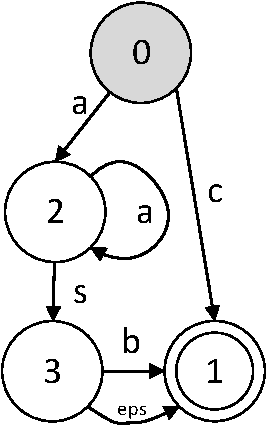
\includegraphics[scale=.5]{pictures/G0initialAutomaton.pdf}
        \label{fig:initialAutomatonsForG0}
    }
    ~
    \subfloat[RA $R_0$ for $G_0$]{
        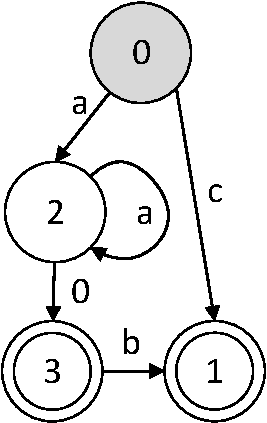
\includegraphics[scale=.5]{pictures/G0minimizedAutomaton.pdf}
        \label{fig:RAForG0}
    }
    \caption{Grammar to RA transformation}
    \label{fig:fig1}
\end{figure}


\subsection{Input Processing}%--------------------------------------------------------------------------------------------------------------------------------------------

In this section we describe changes required in control functions of basic GLL algorithm to handle ECFG.
Main loop is similar to basic GLL one: at each step the main function \textbf{parse} dequeues next descriptor to be processed.
Suppose that current descriptor is a tuple ($C_S, C_U, C_i, C_N$), where $C_S$ --- state of RA, $C_U$ --- GSS node, $C_i$ --- position in the input string $\omega$, and $C_N$ --- SPPF node. 
It is possible to get the following nonexclusive cases during this descriptor processing.

\begin{itemize} 
\item $C_S$ is a final state. Perform pop action (call \textbf{pop} function), because processing of nonterminal is finished.
\item There is a terminal transition $C_S \xrightarrow[]{\omega.[C_i]} q$. 
Move right: create descriptor with state $ q $ and position ($ C_i + 1 $).
Enqueue it regardless of whether it has been created before.
\item There are nonterminal transitions from $C_S$.
It means that processing of new nonterminal should be started, thus new GSS nodes should be created.
To do it, \textbf{create} function should be called for each transition.
It performs necessary operations with GSS and checks if there is an already created SPPF node for the current input position and nonterminal.
\end{itemize}

All required functions are presented below.
Function \textbf{add} enqueues descriptor if it has not already been created, and this function has not been changed.

\begin{algorithmic}    
\Function{create}{$S_{call}, S_{next}, u, i, w$}
    \State $A \gets \Delta(S_{call})$
    \If{($\exists$ GSS node labeled $(A, i)$)}  
    
        \State $v \gets$ GSS node labeled $(A, i)$
        \If{(there is no GSS edge from $v$ to $u$ labeled ($S_{next},w$))}
            \State add GSS edge from $v$ to $u$ labeled ($S_{next},w$)
            \For{($(v, z) \in \mathcal{P} $)}
                \State $(y,N) \gets$ \textbf{getNodes}($S_{next}, u.nonterm, w, z$)
                
                \State $(\_, \_, h) \gets y$
                \State \textbf{add}($S_{next} , u, h, y$)
                
                \If{$N \neq \$$}
                    \State $(\_, \_, h) \gets N$
                    \State \textbf{pop}$(u,h,N)$ 
                \EndIf
            \EndFor
        \EndIf
    \Else
        \State $v \gets$ \textbf{new} GSS node labeled $(A, i)$
        \State create GSS edge from $v$ to $u$ labeled ($S_{next}, w$)
        \State \textbf{add}($S_{call}, v, i, \$ $)
    \EndIf
    \Return{$v$}
\EndFunction
\end{algorithmic}  

\begin{algorithmic}   
\Function{pop}{$u,i,z$}
    \If{($(u,z) \notin \mathcal{P}$)}  
        \State $\mathcal{P}.add(u,z)$
        \ForAll{GSS edges $(u,S,w,v)$}
            \State $(y,N) \gets$ \textbf{getNodes}($S, v.nonterm, w, z$)
            \If{$N \neq \$$}
                \ \textbf{pop}$(v,i,N)$ 
            \EndIf
            
            \If{$y \neq \$$}
                \ \textbf{add}($S,v,i,y$)
            \EndIf
        \EndFor
    \EndIf
\EndFunction
\end{algorithmic}

%\textbf{Pop} function is called when we reach final state. It queues descriptors for all outgoing edges from current GSS node.

\begin{algorithmic}
\Function{parse}{}
    \State $R.add(StartState, new GSSnode(StartNonterminal,0), 0, \$)$
    \While{$R \neq \varnothing $}
    \State{$(C_{S},C_{U},C_{i},C_{N}) \gets R.Get()$}
    \State{$C_{R} \gets \$$}
    
    \If{$(C_{N} = \$) \& (C_{S}$ is final state)}
    \State $eps \gets \textbf{getNodeT}(\varepsilon, C_{i})$  
    \State $(\underline{\hspace{0.25cm}}, N) \gets \textbf{getNodes}(C_{S},C_{U}.nonterm, \$, eps)$
    \State \textbf{pop}$(C_{U},C_{i},N)$ 
    \EndIf
    
    \For{\textbf{each} $transition (C_{S},label,S_{next})$}
        \Switch{$label$}  
        \Case{$Terminal(x)$ where ($x = input[i]$)}
            \State $R \gets \textbf{getNodeT}(x, C_{i})$
            
            \State $(y, N) \gets \textbf{getNodes}(S_{next},C_{U}.nonterm, C_{N}, R)$
            \If{$N \neq \$$}
                \State \textbf{pop}$(C_{U},i+1,N)$ 
            \EndIf
            
            \State $R.add(S_{next}, C_{U}, i + 1, y)$
            
        \EndCase
    
        \Case{$Nonterminal(S_{call})$}
    %\State{$slots \gets pTable[A][input[i]]$}
    %\If{$slots \neq \varnothing$}
            \State \textbf{create}($S_{call}, S_{next}, C_{U}, C_{i}, C_{N}$)
    %\EndIf
    %\ForAll{$L \in slots$}
    %    \State{\Call{add}{L,u,i,\$}} 
    %\EndFor
        \EndCase
        \EndSwitch
        
    \EndFor
    \EndWhile
\EndFunction
\end{algorithmic}



\subsection{Parse Forest Construction}

Result of the parsing process is a structural representation of the input --- a derivation tree, or parse forest in case of multiple derivations.

First, we should define derivation tree for recursive automaton: it is an ordered tree whose root is labeled with the start state,
leaf nodes are labeled with terminals or $\varepsilon$, and interior nodes are labeled with  nonterminals $N$ and their children for a sequence of transition labels of a path in the
automaton which starts from the state $q_i$, where $ \Delta(q_i) = N $.

\begin{mydef}

Derivation tree of sentence $\alpha$ for the recursive automaton $R=(\Sigma, Q, S, F, \delta)$:%grammar $G=(\Sigma, N, S, P)$:

\begin{itemize}
\item Ordered rooted tree; root is labeled with $\Delta(S)$;
\item Leaves are terminals $a\in \Sigma$;
\item Nodes are nonterminals $A\in \Delta(Q)$;
\item Node with label $N_i \in \Delta(q_i)$ has children $l_0 \dots l_n (l_i \in \Sigma \cup \Delta(Q))$ iff there exists a
path $q_i \xrightarrow[]{l_0} q_{i+1} \xrightarrow[]{l_1} \dots \xrightarrow{l_n} q_m$, $q_m \in F$. 
\end{itemize}

\end{mydef}

For arbitrary grammars, RA can be ambiguous in terms of accepted paths, and, as a result, it is possible to get multiple derivation trees for one input string.
Shared Packed Parse Forest (SPPF)~\cite{SPPF} can be used as a compact representation of all possible derivation trees.
We use the binarized version of SPPF, which is proposed in~\cite{brnglr}, in order to decrease memory usage and achieve cubic worst-case time and space complexity.
Binarized SPPF can be used in GLL~\cite{scott2013gll} and contains the following types of nodes (here $i$ and $j$ are the start and the end of derived substring in terms of positions in the input string):

\begin{itemize}
\item Packed nodes are of the form $(S, k)$, where $S$ is a state of automaton, k --- start of derived substring of right child.
Packed node necessarily has a right child node --- symbol node, and optional left child node --- symbol or intermediate node.
\item Symbol nodes have labels $(X, i, j)$ where $X \in \Sigma \cup \Delta(Q) \cup \{\varepsilon\}$.
Terminal symbol nodes ($X \in \Sigma \cup \{\varepsilon\}$) are leaves. 
Nonterminal nodes ($X \in \Delta(Q)$) may have several packed children nodes. 
\item Intermediate nodes have labels $ (S, i, j) $, where $S$ is a state of automaton, and may have several packed children nodes. 
\end{itemize}

Let us describe modifications of original SPPF construction functions.
The function \textbf{getNodeT$(x,i)$} which creates terminal nodes is reused without any modification from basic algorithm.
To handle nondeterminism in states, we define function \textbf{getNodes} which checks if the next state of RA
is final and, if that is case, constructs nonterminal nodes in addition to the intermediate one.
It uses modified function \textbf{getNodeP}: instead of grammar slot it takes separately a 
state of RA and symbol for new SPPF node: current nonterminal or the next RA state.

\begin{algorithmic}
\Function{getNodes}{$S, A, w, z$}
    \If{($S$ is final state)}
        \State $x \gets \textbf{getNodeP}(S, A, w, z)$
    \Else
        \State $x \gets \$ $
    \EndIf
    %\Statex
    %\If{$S.outedges = \varnothing$}
    %    \State $y \gets \$$
    %\Else
        \If{$(w = \$) \&$ not ($z$ is nonterminal node and it's extents are equal)}
            \State $y \gets z$
        \Else
            \State $y \gets \textbf{getNodeP}(S, S, w, z)$
        \EndIf
    %\EndIf
    
    \State \Return{$(y,x)$}
\EndFunction   
\end{algorithmic}
\begin{algorithmic}
\Function{getNodeP}{$S, L, w, z$}
    \State $(\underline{\hspace{0.25cm}}, k, i) \gets z$
    
    \If{($w \neq \$$)}
        \State $(\underline{\hspace{0.25cm}}, j, k) \gets w$
    
        \State $y \gets$ find or create SPPF node labelled $(L, j, i)$  
    
        \If{($\nexists$ child of $y$ labelled $(S, k)$)}
            \State $y\prime \gets \textbf{new}$ $packedNode(S, k)$
            \State $y\prime.addLeftChild(w)$
            \State $y\prime.addRightChild(z)$
            \State $y.addChild(y\prime)$
        \EndIf
    
    \Else
        \State $y \gets$ find or create SPPF node labelled $(L, k, i)$ 
        \If{($\nexists$ child of $y$ labelled $(S, k)$)}
            \State $y\prime \gets \textbf{new}$ $packedNode(S, k)$
            \State $y\prime.addRightChild(z)$
            \State $y.addChild(y\prime)$
        \EndIf
    \EndIf
    \State \Return{$y$}
\EndFunction
\end{algorithmic}

Let us demonstrate an SPPF example for ECFG grammar $G_0$~(fig.~\ref{fig:grammarG0}).
This grammar contains constructions (option symbols and repetition) that should be converted with the use of extra nonterminals to build regular GLL parser.
Our generator constructs recursive automaton $R_0$~(fig.~\ref{fig:RAForG0}) and parser for it.
Possible trees for input $aacb$ \ are shown in fig.~\ref{fig:treesForG0}.
SPPF build by parser~(fig.~\ref{fig:SPPFForG0}) combines all of them.

\begin{figure}[ht]   
    \centering
    \subfloat[Possible derivation trees for $R_0$ and input $ aacb $]{
        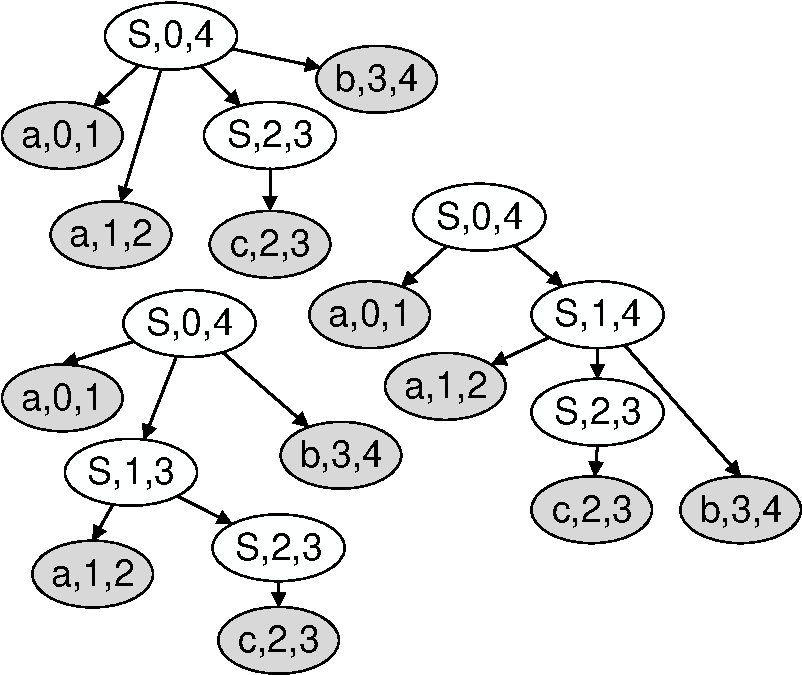
\includegraphics[scale=.5]{pictures/G0trees.pdf}
        \label{fig:treesForG0}
    }
    ~
    \subfloat[SPPF for $R_0$ and input $ aacb $]{
        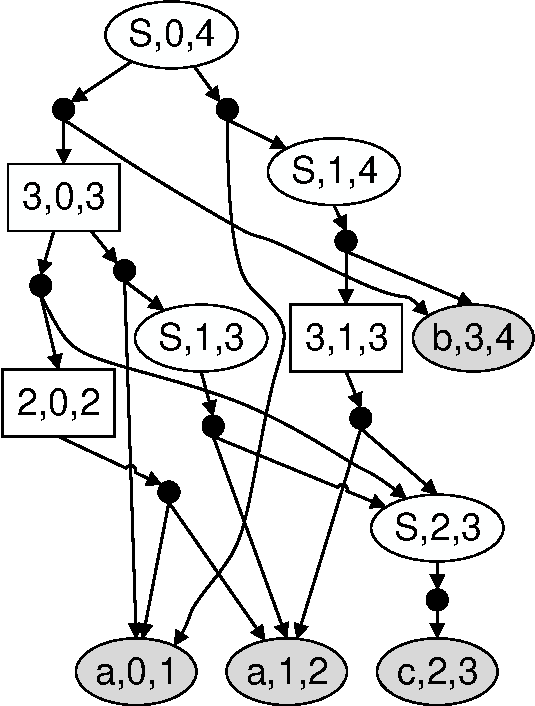
\includegraphics[scale=.5]{pictures/G0SPPF.pdf}
        \label{fig:SPPFForG0}
    }
    \caption{Example for input $ aacb $}
    \label{fig:fig2}
\end{figure}


\section{Evaluation}

We have compared our parsers built on factorized grammar and on minimized recursive automaton.
Grammar $G_1$~(fig.~\ref{fig:grammarG1}) was used for the tests, it has long tails in alternatives which are not unified with factorization.
FSA built for this grammar is presented in fig.~\ref{fig:automatonForG1}.

\begin{figure}[ht]   
    \centering
    \subfloat[Grammar $G_1$]{
        $
        \begin{array}{rl}
        S ::=& K\ (K\ K\ K\ K\ K \ |\ a\ K\ K\ K\ K) \\
        K ::=& S\ K\ |\ a\ K\ |\ a \\
        \end{array}
        $
        \label{fig:grammarG1}
    }

    \subfloat[RA for grammar $G_1$]{
        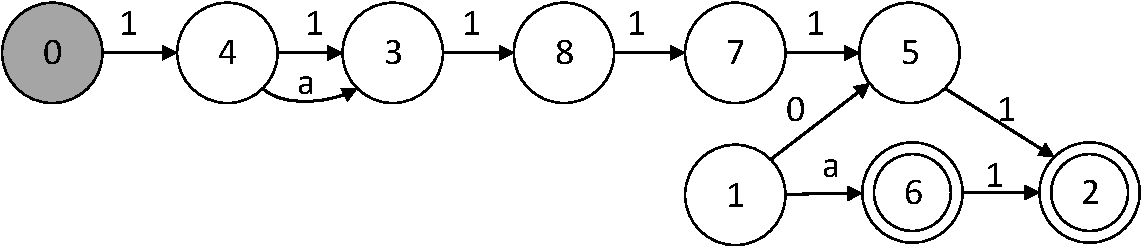
\includegraphics[scale=.5]{pictures/G1automaton.pdf}
        \label{fig:automatonForG1}
    }
    \caption{Grammar $G_1$ and RA for it}
\end{figure}

For this grammar parser for RA should create less GSS edges because the tails of alternatives in producions
are represented by the only path in RA. This fact leads to decrease of SPPF nodes and descriptors.

Experiments were performed on inputs of different length and are presented in fig.~\ref{expPlots}.
Exact values for the input $a^{40}$ are shown in the table~\ref{expTable}.

All tests were run on a PC with the following characteristics:
\begin{itemize}
    \item OS: Microsoft Windows 10 Pro x64
    \item CPU: Intel(R) Core(TM) i7-4790 CPU @ 3.60GHz, 3601 Mhz, 4 Cores, 4 Logical Processors
    \item RAM: 32 GB
\end{itemize}

\begin{table}[ht]   
\begin{center}
    \begin{tabular}{ | c | c | c | c | c | c | }
        \hline
                           & Time, s & Descriptors & GSS Edges & GSS Nodes & SPPF Nodes   \\ \hline
        Factorized grammar & 81.814  & 7940        & 6974      & 80        & 111127244  \\ \hline
        Minimized RA       & 54.637  & 5830        & 4234      & 80        & 74292078  \\ \hline
    \end{tabular}
\end{center}
\caption{Experiments results for input $a^{40}$}
\label{expTable}
\end{table}


\begin{figure}
	\centering
	\subfloat[Number of GSS edges.]{
		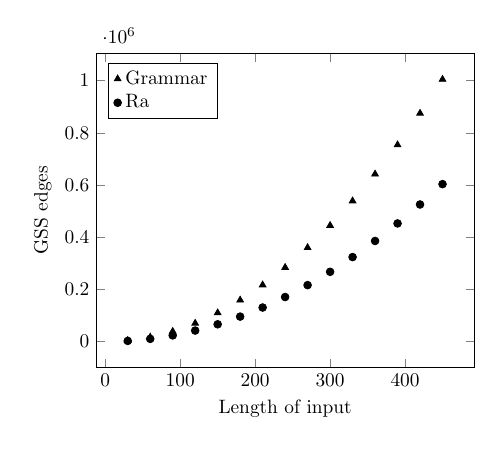
\begin{tikzpicture}[scale=.7]
		\begin{axis}[
		legend cell align=left,
		legend pos = north west,
		xlabel = {Length of input},
		ylabel = {GSS edges},
		%ymode=log
		]
		\addplot [only marks, mark=triangle*] coordinates {
			(30,4022) (60,17012) (90,39002) (120,69992) (150,109982) (180,158972) (210,216962) (240,283952) (270,359942) (300,444932) (330,538922) (360,641912) (390,753902) (420,874892) (450,1004882)
		};
		\addplot [only marks, mark=*] coordinates {
			(30,2452) (60,10282) (90,23512) (120,42142) (150,66172) (180,95602) (210,130432) (240,170662) (270,216292) (300,267322) (330,323752) (360,385582) (390,452812) (420,525442) (450,603472)
		};
		\legend{ 
			Grammar, 
			Ra
		};
		\end{axis}
		\end{tikzpicture}
		\label{fig:GSSedges}
	}
	~
	\subfloat[Time of parsing.]{
		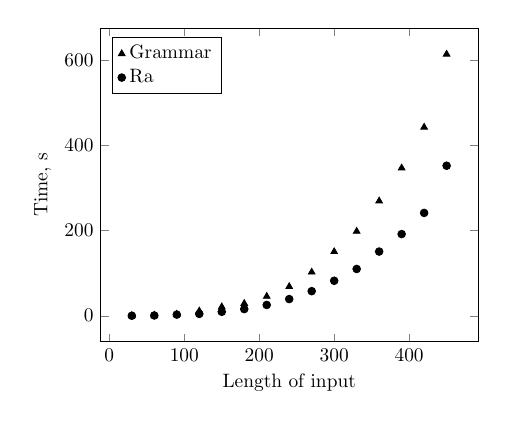
\begin{tikzpicture}[scale=.7]
		\begin{axis}[
		legend cell align=left,
		legend pos = north west,
		xlabel = {Length of input},
		ylabel = {Time, s},
		%ymode=log
		]
		\addplot [only marks, mark=triangle*] coordinates {
			(30,00.1690245) (60,01.1310924) (90,03.6899218) (120,11.1006359) (150,20.8163584) (180,28.7973458) (210,45.3640866) (240,68.3269546) (270,102.2953852) (300,150.2681210) (330,197.9508999) (360,269.1387530) (390,346.4999998) (420,442.0947044) (450,613.3386222)
		};
		\addplot [only marks, mark=*] coordinates {
			(30,00.0625041) (60,00.6562026) (90,02.6719009) (120,04.3594156) (150,09.2969549) (180,15.6406979) (210,25.3438039) (240,39.1251338) (270,57.6720586) (300,82.0470354) (330,109.7031754) (360,150.5466896) (390,191.5317906) (420,241.1571067) (450,351.8283519)
		};
		\legend{ 
			Grammar, 
			Ra
		};
		\end{axis}
		\end{tikzpicture}
		\label{fig:Time}
	}
	
	\subfloat[Number of SPPF nodes.]{
		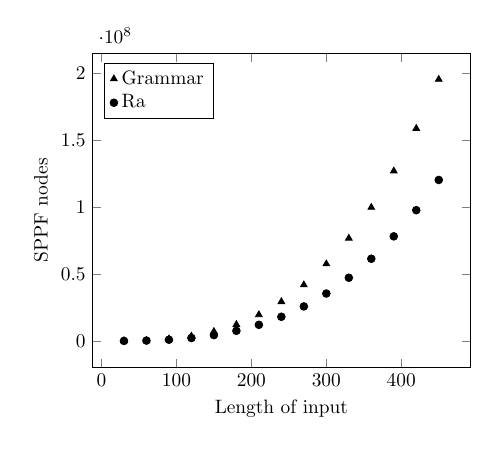
\begin{tikzpicture}[scale=.7]
		\begin{axis}[
		legend cell align=left,
		legend pos = north west,
		xlabel = {Length of input},
		ylabel = {SPPF nodes},
		%ymode=log
		]
		\addplot [only marks, mark=triangle*] coordinates {
			(30,49430) (60,429210) (90,1490290) (120,3583670) (150,7060350) (180,12271330) (210,19567610) (240,29300190) (270,41820070) (300,57478250) (330,76625730) (360,99613510) (390,126792590) (420,158513970) (450,195128650)
		};
		\addplot [only marks, mark=*] coordinates {
			(30,30695) (60,264835) (90,918375) (120,2207315) (150,4347655) (180,7555395) (210,12046535) (240,18037075) (270,25743015) (300,35380355) (330,47165095) (360,61313235) (390,78040775) (420,97563715) (450,120098055)
		};
		\legend{ 
			Grammar, 
			Ra
		};
		\end{axis}
		\end{tikzpicture}
		\label{fig:SPPFnodes}
	}
	~
	\subfloat[Memory usage]{
		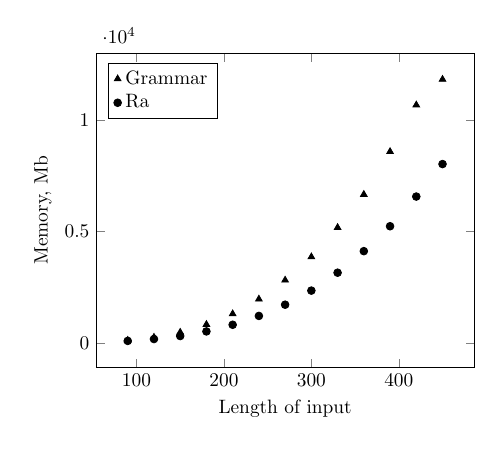
\begin{tikzpicture}[scale=.7]
		\begin{axis}[
		legend cell align=left,
		legend pos = north west,
		xlabel = {Length of input},
		ylabel = {Memory, Mb},
		%ymode=log
		]
		\addplot [only marks, mark=triangle*] coordinates {
			(90,130) (120,267) (150,491) (180,842) (210,1318) (240,1977) (270,2827) (300,3869) (330,5183) (360,6665) (390,8583) (420,10671) (450,11818)
		};
		\addplot [only marks, mark=*] coordinates {
			(90,106) (120,190) (150,325) (180,531) (210,829) (240,1225) (270,1728) (300,2359) (330,3161) (360,4126) (390,5242) (420,6571) (450,8026)
		};
		\legend{ 
			Grammar, 
			Ra
		};
		\end{axis}
		\end{tikzpicture}
		\label{fig:Memory}
	}
	
	\subfloat[Number of descriptors.]{
		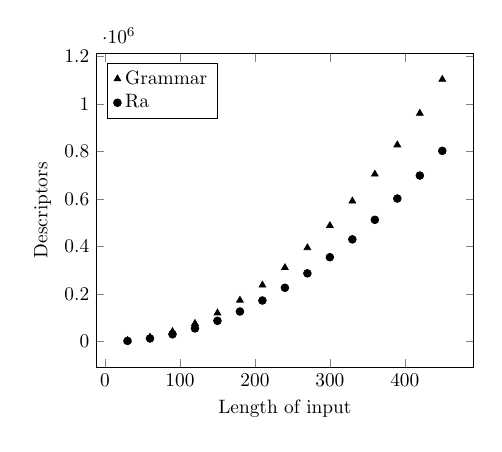
\begin{tikzpicture}[scale=.7]
		\begin{axis}[
		legend cell align=left,
		legend pos = north west,
		xlabel = {Length of input},
		ylabel = {Descriptors},
		%ymode=log
		]
		\addplot [only marks, mark=triangle*] coordinates {
			(30,4346) (60,18551) (90,42656) (120,76661) (150,120566) (180,174371) (210,238076) (240,311681) (270,395186) (300,488591) (330,591896) (360,705101) (390,828206) (420,961211) (450,1104116)
		};
		\addplot [only marks, mark=*] coordinates {
			(30,3181) (60,13531) (90,31081) (120,55831) (150,87781) (180,126931) (210,173281) (240,226831) (270,287581) (300,355531) (330,430681) (360,513031) (390,602581) (420,699331) (450,803281)
		};
		\legend{ 
			Grammar, 
			Ra
		};
		\end{axis}
		\end{tikzpicture}
		\label{fig:Descriptors}
	}
	\caption{Experiments results.}
	\label{expPlots}
\end{figure}

Results of performed experiments agree with the fact that on some grammars our approach 
shows better results than parsers built on factorized grammars.
With grammar $G_1$ in general minimized RA version works $33\%$ faster, uses $27\%$ less descriptors, $29\%$ less GSS edges
and $33\%$ less SPPF nodes.

\section{Conclusion and Future Work}

Described algorithm and parser generator based on it are implemented in F\# programming language as a part of the YaccConstructor project.
Source code is available here:~\url{https://github.com/YaccConstructor/YaccConstructor}.

As we showed in evaluation, proposed modification not only increases performance, but also decreases memory usage. 
It is crucial for big input processing.
For example, Anastasia Ragozina in her master's thesis~\cite{ragozina} shows that GLL can be used for graph parsing.  
Some areas deal with big graphs, for example, metagenomic assemblies in bioinfomatics and social graphs.
We hope that using the proposed modification we can improve performance of graph parsing algorithm too. 
We perform some tests that demonstrate performance increase in metagenomic analysis, but further integration with graph parsing is required.

One of the ways to specify semantic of language is attributed grammars, but it is not supported in the algorithm which is presented in this article.
There is a number of works on subclasses of attributed ECFGs (for example~\cite{AttributedELL}), however still there is no general solution for arbitrary ECFGs.
Thus, arbitrary attributed ECFGs and semantic calculation support is a work for future.

Another question is a possibility of unification of our results with tree languages theory: our definition of derivation tree for ECFG is quite similar to unranked tree and SPPF is similar to automata for unranked trees~\cite{TATA}.
Theory of tree languages seems to be more mature than theory of SPPF manipulations in general.
Moreover some relations between tree languages and ECFG are discussed in the paper~\cite{TreeLangAndECFG}.
We hope that the investigation of relations between tree languages and SPPF may produce interesting results.


\bibliographystyle{abbrv}
\bibliography{bibliography}
\section{Dataset description}\label{section:dataset}

In our evaluation we use dataset which contains the following parts.
{\setlength{\tabcolsep}{0.4em}
	\begin{table}[h]
		\caption{RDFs properties}
		\label{tbl:propRDF}
		\rowcolors{2}{}{lightgray}
		\begin{tabular}{| l | c | c | c | c |}
			\hline
			Name                  & \#V    & \#E     & \#type &\#subClassOf \\
			\hline
			\hline
			atom-primitive				& 291		& 685		& 138	& 122	\\
			univ-bench					& 179		& 413		& 84		& 36		\\
			travel						& 131		& 397		& 90		& 30		\\
			skos							& 144		& 323		& 70		& 1		\\
			people\_pets					& 337		& 834		& 161	& 33		\\
			generations					& 129		& 351		& 78		& 0		\\
			foaf							& 256		& 815		& 174	& 10		\\
			biomed-mesure-prim   	    & 341		& 711		& 130	& 122	\\
			funding						& 778		& 1480		& 304	& 90               \\
			pizza						& 671		& 2604		& 365	& 259              \\
			wine							& 733		& 2450		& 485	& 126              \\
			core							& 1323		& 8684		& 1412	& 178              \\
			pathways						& 6238		& 37196		& 3118 	& 3117             \\
			go-hierarchy					& 45007		& 1960436	& 0		& 490109           \\
			enzyme						& 48815		& 219390		& 14989	& 8163             \\
			eclass\_514en				& 239111		& 1047454	& 72517	& 90962            \\
			go							& 272770		& 1068622	& 58483	& 90512            \\
			\hline
		\end{tabular}
	\end{table}
}

{\setlength{\tabcolsep}{0.4em}
\begin{table*}[h]
\caption{RDFs query $G_2$ (time is measured in seconds and memory is measured in megabytes)}
\label{tbl:tableRDFQ2}
\rowcolors{3}{}{lightgray}
\begin{tabular}{| l | r  r | r  r | r  r | r  r | r  r |}
    \hline

    \multirow{3}{*}{Name}   &   \multicolumn{6}{|c|}{Relational semantics index}	&	\multicolumn{4}{|c|}{Single path semantics index} \\
    \cline{2-11}
    &	\multicolumn{2}{|c|}{RG\_CPU\textsubscript{rel}}	&	\multicolumn{2}{|c|}{RG\_CUSP\textsubscript{rel}}	&	\multicolumn{2}{|c|}{RG\_SPARSE\textsubscript{rel}} &	\multicolumn{2}{|c|}{RG\_CPU\textsubscript{path}}	&	\multicolumn{2}{|c|}{RG\_SPARSE\textsubscript{path}}	 \\
    \cline{2-11}
    &   Time & Mem &  Time     & Mem & Time     & Mem  &  Time     & Mem & Time     & Mem \\
    \hline
    \hline
    atom-primitive          & 0.001 & 0.3  & 0.001 & 0.1 & 0.002 & 0.1   & 0.001 & 0.3  & 0.002 & 0.1   \\
biomedical-mesure-primitive & 0.002 & 0.1  & 0.014 & 2.0   & 0.009 & 0.1   & 0.006 & 0.1  & 0.012 & 0.1   \\
core                        & 0.001 & 0.3  & 0.006 & 0.1 & 0.004 & 0.1   & 0.003 & 0.3  & 0.005 & 0.1   \\
eclass\_514en               & 0.035 & 6.5  & 0.020 & 16.0  & 0.100   & 12.0    & 0.123 & 17.7 & 0.127 & 18.0    \\
enzyme                      & 0.006 & 3.9  & 0.006 & 0.6 & 0.010  & 0.1   & 0.012 & 5.3  & 0.008 & 0.4   \\
foaf                        & 0.001 & 0.1  & 0.004 & 0.1 & 0.002 & 0.1   & 0.001 & 0.1  & 0.003 & 0.1   \\
funding                     & 0.002 & 0.1  & 0.015 & 0.4 & 0.007 & 0.1   & 0.009 & 0.1  & 0.008 & 0.1   \\
generations                 & 0.001 & 0.1  & 0.001 & 0.1 & 0.001 & 0.1   & 0.001 & 0.1  & 0.001 & 0.1   \\
go-hierarchy                & 0.095 & 17.8 & 0.253 & 528.0 & 0.175 & 130.4 & 0.884 & 88.8 & 0.306 & 138.8 \\
go                          & 0.306 & 25.8 & 0.240 & 84.0  & 0.181 & 25.4  & 0.918 & 78.1 & 0.219 & 34.2  \\
pathways                    & 0.005 & 0.2  & 0.005 & 0.4 & 0.004 & 0.1   & 0.017 & 0.5  & 0.003 & 0.1   \\
people\_pets                & 0.001 & 0.1  & 0.007 & 0.1 & 0.004 & 0.1   & 0.001 & 0.1  & 0.005 & 0.1   \\
pizza                       & 0.002 & 0.3  & 0.012 & 0.2 & 0.008 & 0.1   & 0.010  & 0.3  & 0.009 & 0.1   \\
skos                        & 0.001 & 0.1  & 0.001 & 0.1 & 0.001 & 0.1   & 0.001 & 0.1  & 0.002 & 0.1   \\
travel                      & 0.001 & 0.1  & 0.007 & 0.1 & 0.005 & 0.1   & 0.001 & 0.1  & 0.005 & 0.1   \\
univ-bench                  & 0.001 & 0.1  & 0.007 & 0.1 & 0.005 & 0.1   & 0.001 & 0.1  & 0.005 & 0.1   \\
wine                        & 0.001 & 0.3  & 0.006 & 0.1 & 0.004 & 0.1   & 0.002 & 0.3  & 0.004 & 0.1  \\
    \hline
  \end{tabular}
\end{table*}
}

\begin{itemize}
\item The real-world data RDFs provided in CFPQ\_Data dataset\footnote{CFPQ\_Data dataset GitHub repository: \url{https://github.com/JetBrains-Research/CFPQ_Data}. Access date: 12.11.2019.} from~\cite{Mishin:2019:ECP:3327964.3328503}.
\item Geospecies (RDF which contains information about biological hierrarchy\footnote{The Geospecies RDF: \url{https://old.datahub.io/dataset/geospecies}. Access date: 12.11.2019.} and same-generation query over \textit{broaderTransitive} relation) is provided in~\cite{Kuijpers:2019:ESC:3335783.3335791} and integrated in our evaluation with CFPQ\_Data.
\item It was shown in~\cite{Mishin:2019:ECP:3327964.3328503} that matrix-based algorithm is performant enough to handle bigger RDFs than those used in the initial datasets, such as~\cite{RDF}.
So, we add several big RDFs to CFPQ\_Data and use them in our evaluation.
New RDFs: \textit{go-hierarchy, go, enzime, core, pathways} are from UniProt database\footnote{Protein sequences data base: \url{https://www.uniprot.org/}. RDFs with data are avalable here: \url{ftp://ftp.uniprot.org/pub/databases/uniprot/current_release/rdf}. Access date: 12.11.2019}, and \textit{eclass-514en} is from eClassOWL project\footnote{eClassOWL project: \url{http://www.heppnetz.de/projects/eclassowl/}. eclass-514en file is available here: \url{http://www.ebusiness-unibw.org/ontologies/eclass/5.1.4/eclass_514en.owl}. Access date: 12.11.2019.}.
\end{itemize}

The properties of the RDFs from the dataset are given in table \ref{tbl:propRDF}. 
Geospecies RDF contains 450609 vertices, 2311461 edges, and 20867 edges labeled by \textit{broaderTransitive}.
Note that while the number of edges labeled by \textit{broaderTransitive} is equal to provided in~\cite{Kuijpers:2019:ESC:3335783.3335791}, the total number of vertices and edges is bigger. It is because we naively convert each triple from RDF to edge in the graph, while J. Kuijpers et al. use special \textit{neosemantics}\footnote{Neosemantix is an RDF processing plugin for Neo4j. Web page: \url{https://neo4j.com/labs/nsmtx-rdf/}. Access date: 30.03.2020.} plugin which can, for example, handling multivalued properties accurately.  

The variants of the \textit{same-generation query}~\cite{FndDB} are used in almost all cases because it is an important example of real-world queries that are context-free but not regular.
So, variations of the same generation query are used in our evaluation.
All queries are added to the CFPQ\_Data dataset.

We use two queries over \textit{subClassOf} and \textit{type} relations.
The first query is the grammar $G_1$:
\[
 \begin{array}{lcl}
   s  \rightarrow \textit{subClassOf}^{\ -1} \ s \ \textit{subClassOf}   & \quad & s  \rightarrow \textit{type}^{\ -1} \ s \ \textit{type}     \\
   s  \rightarrow \textit{subClassOf}^{\ -1} \ \textit{subClassOf}       & \quad & s  \rightarrow  \textit{type}^{\ -1}  \ \textit{type}

 \end{array}
 \]
The second one is the grammar $G_2$: \[s \rightarrow \textit{subClassOf}^{\ -1} \ s \ \textit{subClassOf} \mid \textit{subClassOf}\]

For geospecies we use same-generation query \textit{geo} from the original paper~\cite{Kuijpers:2019:ESC:3335783.3335791}: \[s \rightarrow \textit{broaderTransitive} \ s \ \textit{broaderTransitive}^{\ -1} \]
\[s \rightarrow \textit{broaderTransitive}  \ \textit{broaderTransitive}^{\ -1} \]


\section{Evaluation Details}

Results for RDFs querying with $G_2$ grammar are presented in table~\ref{tbl:tableRDFQ2}.
We can see, that for small graphs time for both relational and single-path querying are similar for CPU and GPGPU versions, but for bigger graphs (\textit{go} and \textit{go-hierarchy}, for example) GPUPU version is more performant than CPU one.

\balance


\end{document}
